\chapter{Background}
\vspace{1cm}

Background blah.

\section{File Systems}

\todo{Find reference for basic file system stuff.}

The file system is a fundamental abstraction for almost all modern operating
systems. The abstraction allows the operating system and user programs to
interact with a variety of devices and services through a single unified
interface.
The purpose of a specific file system is to implement this common interface for
a particular underlying data store. The exact nature of the data store is not
important to the consumer of the file system's interface. The underlying data
store is commonly a physical storage device such as a hard disk drive (HDD).
However, it is important to note that this is not always the case and there is
no requirement for a file system to manage a physical storage device. File
systems that depend on another file system as their underlying data store are
known as a VFS (virtual file system).

The high level filing cabinet metaphor that is built on the low level interface
provided by a particular file system implementation will be familiar to most
computer users. The metaphor consists of a filing cabinet containing many named
files. These files can contain arbitrary data. However, some of these files may
not contain data themselves but rather other files, and in this case they are
called directories (or folders in some versions of the metaphor). This nesting
of files within directories creates a hierarchical structure where a single
root directory (analogous to the filing cabinet) contains an arbitrarily
deeply nested series of files and directories. The hierarchy of files within
directories can conceptually be arbitrarily deep, but most particular
implementations enforce a limit for simplicity. The filing cabinet metaphor is
also useful in demonstrating that a file or directory can only be contained
within one other directory. Each file or directory (excluding the root
directory) must have one and only one parent in the hierarchy.

In Figure~\ref{fig:sample file hierarchy} there are two distinct files named
\texttt{timeline.txt}. It becomes ambiguous to refer to a file only by its name
when this is the case. It is useful to use the steps taken to arrive at a file
or directory to identify it within the file hierarchy. For example, the steps
taken to arrive at \texttt{timeline.txt} would be \texttt{/} then
\texttt{documents} then \texttt{project1} then \texttt{timeline.txt}. This list
of steps is known as a path and can be written as a \texttt{/} delimited list
of the steps taken to reach a file or directory. Using the previous example the
path would be \texttt{/documents/project1/timeline.txt}. As a result of the
single parent rule, each file or directory has a single path that uniquely
identifies it amongst all other files and directories in the hierarchy. This
single unique path is known as an absolute path, meaning the steps to arrive at
a file or directory are completely specified all the way from the root of the
file system\footnote{This is not the case when the file system contains
symbolic links.}. In contrast to this, a relative path is a path that is not
specified from the root of the file system, but from some other arbitrary
location. For example, the path \texttt{project1/timeline.txt} is a relative
path that is specified from the \texttt{documents} directory. The directory
that a relative path is specified from is known as the current working
directory.

The strict hierarchical nature of the file system falls apart with the addition
of links to the file system. There are two types of links in UNIX file systems:
hard links and symbolic (or soft) links. Symbolic links (often abbreviated as
symlinks) are a special kind of file-like object that act as a window into
another part of the file system. Symbolic links have a name like a normal file,
but they additionally have a target which is another path that they act as a
window into. For example, you could imagine a symbolic link named
\texttt{my-link} in the \texttt{images} directory with a target of
\texttt{/code}. The existence of this link would mean that now the path
\texttt{/images/my-link/main.c} refers to the same file as
\texttt{/code/main.c} (the same property holds for
\texttt{/images/my-link/Makefile} also). \todo{Talk about how symbolic links
can introduce cycles.}

A hard link is a reference to a piece of data. Hard links are very similar to
regular files, because regular files are in fact hard links. A hard link
references an inode\footnote{\todo{Explain that even Dennis Ritchie does not
know exactly why an inode is called an inode.}
https://lkml.indiana.edu/hypermail/linux/kernel/0207.2/1182.html}\cite{inode}
by way of an inode number. An inode is a data structure internal to the file
system that is used to keep track of metadata relating to some user data. An
inode number is a number that uniquely identifies an inode on a particular file
system. The consequence of this is that hard links, and therefore regular
files, don't actually own their data; they only reference it through an inode
number. This means that there can be multiple distinct files that reference the
same inode, and therefore are associated with the same data.

% Sample file hierarchy figure {{{
\begin{figure}[h]
\centering
\begin{forest}
    for tree = {%
        folder,
        grow'=0,
        fit=band,
        font=\ttfamily,
        s sep=0.5mm,
        l sep=0.7cm,
    }
    [/,color=teal
        [code,color=teal
            [main.c,color=olive]
            [Makefile,color=olive]
        ]
        [documents,color=teal
            [project1,color=teal
                [timeline.txt,color=olive]
            ]
            [project2,color=teal
                [timeline.txt,color=olive]
            ]
            [projects.txt,color=olive]
        ]
        [images,color=teal
            [scan.jpg,color=olive]
        ]
    ]
\end{forest}
\caption[Sample file hierarchy]{Sample file hierarchy with directories in
    \textcolor{teal}{blue}
    and files in \textcolor{olive}{green}.}
\label{fig:sample file hierarchy}
\end{figure}
% }}}

\subsection{Operating Systems and the File System}

\todo{
    Talk about how ls makes a system call and the kernel receives it and then
    calls the fuse kernel module who then writes to unix socket which fuser
    (Rust) reads who then calls me. In the general case libFUSE would call the
    libc function mount with fs type 'fuse'. In my case fuser calls fusermount3
    and listens to the returned unix socket for messages from the kernel.
}

The primary way most users interact with file systems is through a GUI
(graphical user interface) file manager such as \texttt{thunar} or
\texttt{nautilus}. \todo{Maybe screenshot of file manager with tree view?}
However, it is also possible to manage a file system without a GUI and use CLI
(command line interface) tools such as \texttt{ls} or \texttt{mv}. Both GUI
file managers and CLI tools utilise the low level interface exposed by the
operating system and implemented by a particular file system. The traditional
way to use this interface is via the platform library exposed by the operating
system\footnote{On some platform like Microsoft Windows, using the platform
library is required because the system call interface is not guaranteed to be
stable between releases.}. \todo{Not sure if I should stay abstract about a
particular operating system or be specifically about UNIX-likes here.} On
UNIX-like operating systems this library is \texttt{libc}\cite{libc}. \todo{Do
I need to talk about the difference between an abstract libc and concrete like
glibc or musl?} The overwhelming majority of programs that run on UNIX-like
operating systems use \texttt{libc} to help them interact with the platform.
The operating systems' \texttt{libc} contains functions that require access to
the file system (such as \texttt{stat}\cite{stat-syscall}). To get access to
the file system the \texttt{libc} function will execute a system
call\cite{syscalls} (often called a syscall). A system call is a way for an
unprivileged user program to ask the operating system to perform an action on
its behalf. When executed, a system call performs a context switch
\todo{Explain what a context switch actually is.} and jumps into kernel
code\footnote{This is not strictly true, some system calls do not require jumping
into kernel code.}.
The kernel is the part of the operating system that, amongst many other
functions, responds to system calls. When the kernel responds to a system call
that requires accessing the file system, it must first ascertain which file
system implementation is the correct one to call for this particular action.
On Linux this is the VFS layer in the kernel\cite{kernel-vfs}. Once this is
determined, the kernel asks the file system implementation to perform the
action specified by the system call. It may also return some data to the
calling user program via a buffer or a return value.

\subsection{FUSE File Systems}

% FUSE diagram figure {{{
\begin{figure}[h]
    \centering
    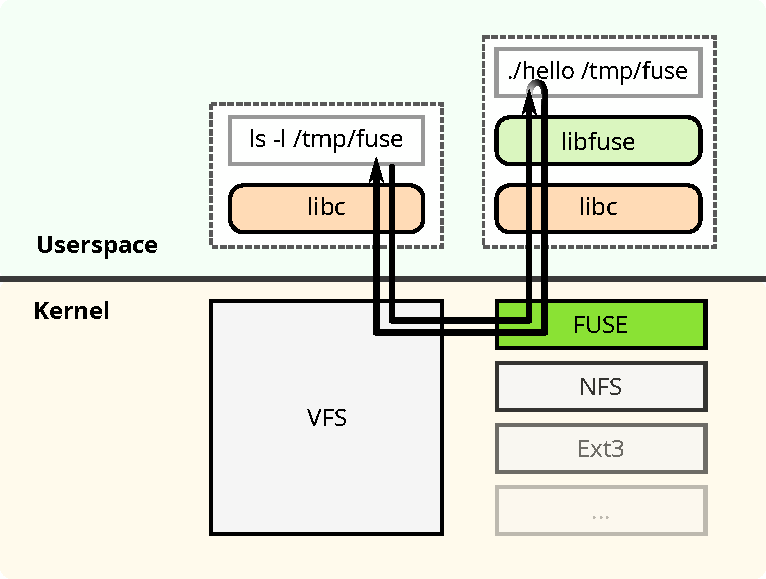
\includegraphics[width=10cm]{../data/fuse.pdf}
    \caption[FUSE Data Flow]{A diagram to show the flow of data in a FUSE file
        system. Taken from \cite{fuse-diagram-source}}
    \label{fig:fuse diagram}
\end{figure}
% }}}

Most file systems are built into the kernel; either directly compiled in or as
kernel modules. This means they will run in kernel mode (ring 0 on x86
platforms). If code running as part of the kernel crashes or hangs, there is a
danger that this could crash or hang the entire system. Additionally, code
running in kernel mode has the power to do anything on the system, so a
security issue in any code run at this level code could result in a compromised
system. To reduce the danger of writing a file system, Linux allows file
systems to be run as userspace processes using a technology called
FUSE\cite{kernel-fuse} (file system in userspace).

Looking at Figure~\ref{fig:fuse diagram}, there are similarities between the
process of accessing a file system built into the kernel (in the diagram NFS
and ext3 are used as an example) and the process of accessing a FUSE file
system. For both built in file systems and FUSE file systems, the calling
program uses \texttt{libc} to ask the kernel to perform a file system action,
and the kernel dispatches the call to the correct file system implementation
using the VFS layer. When the VFS layer requires action from a FUSE file
system, it passes the request to the FUSE kernel module. The FUSE kernel module
then communicates (the nature of the communication and the medium across which
it takes place are discussed in Section~\ref{mounting-fuse-fs}) the request to
the user space process. The user space process can then do whatever it pleases
to generate a response which is then passed back through the layers into the
kernel and back to the calling user space program that made the request.

\todo{Disadvantages of FUSE - slow}

\subsubsection{Mounting FUSE File Systems}
\label{mounting-fuse-fs}

To mount a (non-root) file system means attaching the root of a child file
system to an empty directory in another parent file system. The two file
systems remain entirely independent; their connection is only simulated using
the kernel's VFS layer. However, to other programs it appears that the contents
of the child file system are available as a sub-directory in another parent
file system.

On Linux mounting a file system is a restricted operation that can only be
performed by the root user\cite{mount}. However, FUSE has the explicit goal of
"allowing secure, non-privileged mounts"\cite{kernel-fuse}. To allow FUSE file
systems to be mounted by non-privileged users, FUSE provides a mounting utility
\texttt{fusermount} which is installed with the setuid\cite{setuid} permission
set to the root user. A binary with this permission can be run by a normal
user, but whilst it is running it has all the privileges of the root user. This
allows a normal user to mount a FUSE file system.

After the FUSE file system has been mounted there needs to be a channel for
communication between the FUSE kernel module and the user space program
managing the file system. This channel is the \texttt{/dev/fuse} pseudo device
file. However, reading and writing to this file is a privileged action so
\texttt{fusermount} (with its elevated permissions) is responsible for opening
a handle to \texttt{/dev/fuse} and then returning it to the user space file
system. \texttt{fusermount} returns this handle over a socket given to it via
an environment variable at launch.

\todo{Talk (briefly I think) about the binary protocol fuse talks over
\texttt{/dev/fuse}}

\section{The Rust Programming Language}
